\documentclass{report}
\usepackage[a4paper, portrait, top=20mm, left=10mm, right=10mm, bottom=20mm]{geometry}
\usepackage{graphicx,wrapfig,amsmath,amssymb} 

\title{Probability Theory}
\author{Abhijit Amrendra Kumar}
\date{August 2023}

\begin{document}

\maketitle

\chapter{Introduction}
\section{Axioms}

\begin{itemize}
  \item \textbf{Set}: An unordered collection of unique objects
  \item \textbf{Experiment}: An empirical procedure
  \item \textbf{Statistical/Random Experiment}: An empirical procedure (aka. experiment) with an uncertain outcome
  \item \textbf{Sample Space $\Omega$}: Set of all possible outcomes of a random experiment.
  \item \textbf{Event}: A subset of a sample space
        \begin{itemize}
          \item Operations on events include union $A\cup B$, intersection $A\cap B$, complement $\bar{A}$, and subtraction $A-B$
        \end{itemize}
  \item \textbf{Event space $\beta$}: A set of all possible events that we want to model
        \begin{itemize}
          \item It is a subset of the \textbf{powerset} of the sample space $\Omega$
          \item Includes the empty set $\phi$ and the sample space $\Omega$
          \item It must be closed under countable unions
          \item It must be closed under complementation
          \item It is also referred to as a $\sigma$-algebra
        \end{itemize}
  \item \textbf{Probability Function/Measure $P$}: A function which gives the probability/chance of the occurence of an event.
        \begin{itemize}
          \item $P : \beta \rightarrow [0,1]$
          \item $P(\phi) = 0$
          \item $P(\Omega) = 1$
          \item For pairwise disjoint sets/events $A_1,A_2,...,A_n$, $$P(A_1\cup A_2 \cup ... A_n) = P(A_1) + P(A_2) + ... P(A_n)$$
          \item Operations of probability functions include complement $\bar{P}$, union $A\cup B$, and difference $A-B$
        \end{itemize}
  \item \textbf{Probability Space $(\Omega,\beta,P)$}: A probability space is a triplet $(\Omega,\beta,P)$, where $\Omega$ is the sample space, $\beta$ is the probability space, and $P$ is the probability function.
        \begin{center}
          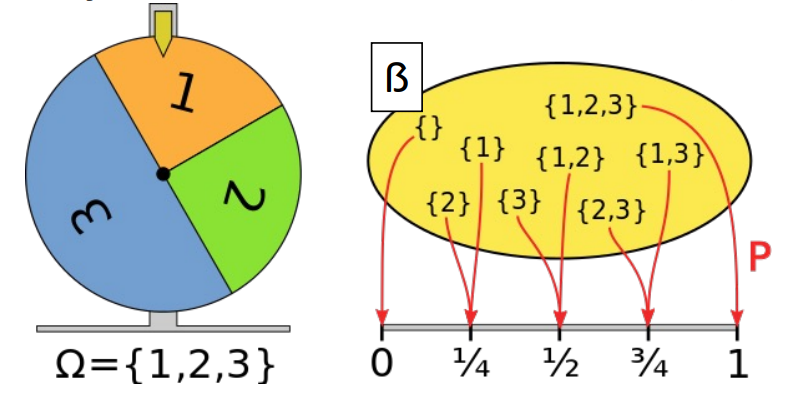
\includegraphics[scale=0.3]{"images/prob-01.png"}
        \end{center}
        \begin{itemize}
          \item Probability Space for 2 Different Kinds of Experiments: $\Omega' = \Omega_1 \times \Omega_2$
          \item Probability Space for Repeated Experiments: $\Omega' = \Omega \times \Omega$
        \end{itemize}
\end{itemize}

\section{Definitions}
\begin{itemize}
  \item \textbf{Population}: A set of similar items or events which is of interest for some question or experiment
  \item \textbf{Sample}: A set of objects collected/selected from a statistical population by a defined procedure
  \item \textbf{Joint Probability}: $P(A \text{ and } B) := P(A,B) := P(A\cap B)$
  \item \textbf{Conditional Probability}: Given an event $B$, the conditional probability of another event $A$ is given by $P(A|B) := P(A\cap B)/P(B)$
  \item \textbf{Partitions}: A set of events $\{B_1,B_2,...,B_n\}$ is a partition of a sample space $\Omega$ if
        \begin{itemize}
          \item the set is mutually exclusive (i.e. $B_i\cap B_j = \phi \forall i\neq j$)
          \item the set is exhaustive (i.e. $\underset{i}{\bigcup}{B_i} = \Omega$)
        \end{itemize}
  \item \textbf{Total Probability}: Given a partition $B = \{B_1,B_2,...B_n\}$, the total probability is given by $$P(A) := \underset{i}{\sum} P(A\cap B_i) = \underset{i}{\sum} P(A|B_i)P(B_i)$$
        \begin{itemize}
          \item The partition $B$ induces a partition over the event A
                \begin{center}
                  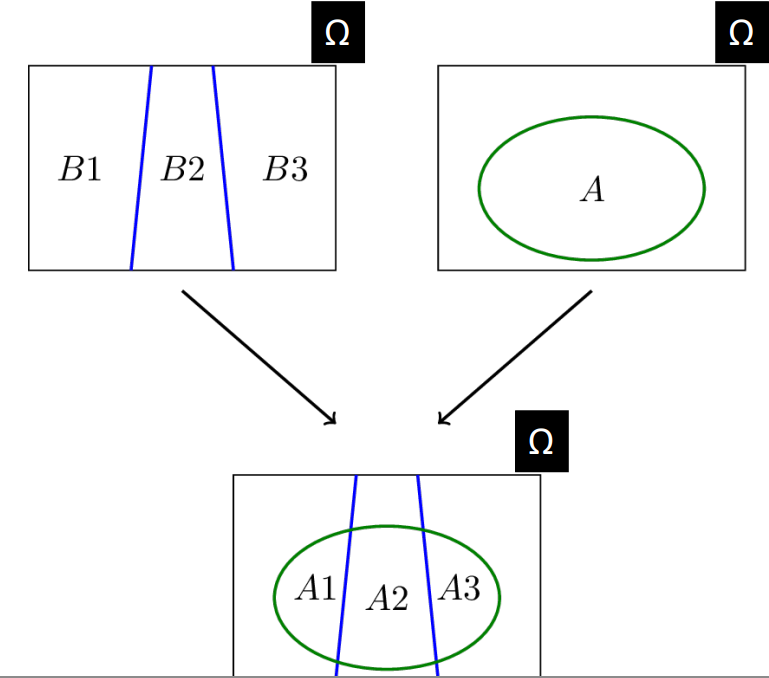
\includegraphics[scale=0.4]{"images/prob-02.png"}
                \end{center}
        \end{itemize}
  \item \textbf{Independent Events}: Two events $A$ and $B$ are independent iff $P(A,B) = P(A)P(B)$
  \item \textbf{Conditional Independence}: Given event $C$, events $A,B$ are conditionally independent iff $$P(A,B|C) := P(A|C)P(B|C)$$
\end{itemize}

\chapter{Random Variable}
\section{Definition}

\noindent A \textbf{random variable} $X$ is a function defined on the probability space $(\Omega,\beta,P)$ that maps each element in the sample space $\Omega$ to a real number $X: \Omega \rightarrow \mathbb{R}$. Random variables are used when we are more interested in the value associated with an outcome instead of the outcome itself. \\

\noindent \textbf{Discrete RV}: $X: \Omega \rightarrow S$, where $S \subset \mathbb{R}$ and the cardinality of the set $|S|$ is countably infinite $|S| \leq |\mathbb{N}|$.

\noindent \textbf{Continuous RV}: $X: \Omega \rightarrow S$, where $S \subset \mathbb{R}$ and the cardinality of the set $|S|$ is uncountably infinite $|S| \leq |\mathbb{R}|$.

\section{Events via Random Variables}

\noindent \textbf{Notation}: Upper case letters (eg. $X$) will be used to denote a random variable, while lowercase letters (eg. $x$) will be used to denote a specific value that can be taken by a random variable. \\

\noindent Examples:
\begin{align*}
  \{X = a\}     & = \{ s \in \Omega : X(s) = a \}     \\
  \{X < a\}     & = \{ s \in \Omega : X(s) < a \}     \\
  \{a < X < b\} & = \{ s \in \Omega : a < X(s) < b \}
\end{align*}

\noindent Using this notation, we can also define event probabilities
\begin{align*}
  P_X(\{X = a\})     & = P(\{ s \in \Omega : X(s) = a \})     \\
  P_X(\{X < a\})     & = P(\{ s \in \Omega : X(s) < a \})     \\
  P_X(\{a < X < b\}) & = P(\{ s \in \Omega : a < X(s) < b \})
\end{align*}

\section{Distribution Functions via Random Variables}
\subsection{Cumulative Distribution Function (CDF)}

\noindent For a real-valued random variable $X$, the CDF is defined as $f_X(x) := P_X(X \leq x)$. \\

\noindent \textbf{Properties of CDF}:
\begin{itemize}
  \item $f$ is monotonically non-decreasing.
  \item $f$ is right-continuous, i.e. $\text{lim}_{\epsilon \rightarrow 0^+} f(x+\epsilon) = f(x), \forall \ x \in \mathbb{R}$
  \item $\text{lim}_{x \rightarrow -\infty} f(x) = 0$
  \item $\text{lim}_{x \rightarrow +\infty} f(x) = 1$
\end{itemize}

\newpage

\noindent \textbf{Theorem}: Let $X$ be a random variable with CDF $f_X$. Then, $$P(a < X \leq b) = f_X(b) - f_X(a)$$

\noindent \textbf{Proof}: We know that
$$\{-\infty < X \leq b\} = \{-\infty < X \leq a\} \cup \{a < X \leq b\} $$

\noindent The two sets on the right side are disjoint, which implies
\begin{align*}
  P_X(-\infty < X \leq b)    & = P_X(X \in \{-\infty < X \leq a\} \cup \{a < X \leq b\}) \\
                             & = P_X(-\infty < X \leq a) + P_X(a < X \leq b)             \\
  \implies P_X(a < X \leq b) & = P_X(X \leq b) - P_X(X \leq a)                           \\
                             & = f_X(b) - f_X(a)
\end{align*}

\hrule
\vspace{5mm}

\noindent \textbf{Theorem}: Let $X$ be a random variable with CDF $f_X$. Then, $$P(X = c) = f_X(c) - f_X(c^-)$$

\noindent \textbf{Proof}: For all $x \in \mathbb{R}$, we have
$$\{x\} = \overset{\infty}{\underset{n=1}{\bigcap}} \bigl(
  x - 1/n, x \bigl]$$

\noindent that is, $\{x\}$ is the limit of a decreasing sequence of sets. Thus we can write
\begin{align*}
  P_X(X = x) & = P_X \Bigl[ \overset{\infty}{\underset{n=1}{\bigcap}} \bigl\{ x - 1/n < X \leq x \bigr\} \Bigr] \\
             & = \underset{n \rightarrow \infty}{\text{lim}} P_X\bigl[x - 1/n < X \leq x \bigr]                 \\
             & = \underset{n \rightarrow \infty}{\text{lim}} \bigl[F_X(x) - F_X(x - 1/n) \bigr]                 \\
             & = F_X(x) - F_X(x^-)
\end{align*}



\end{document}
